\documentclass[12pt]{article}

\usepackage{amsmath}
\usepackage{graphicx}
\usepackage{verbatim} 
\usepackage{color}
\usepackage{subfigure}
\usepackage{hyperref} 
\usepackage{listings}

\begin{document}

\section{Assignment 1: Projection Error}

\subsection{Implemation}
Implemeted a general Gaussian formel for standard beam 

\subsection{Resultat}

\subsubsection{A: Paraxial Approximation}
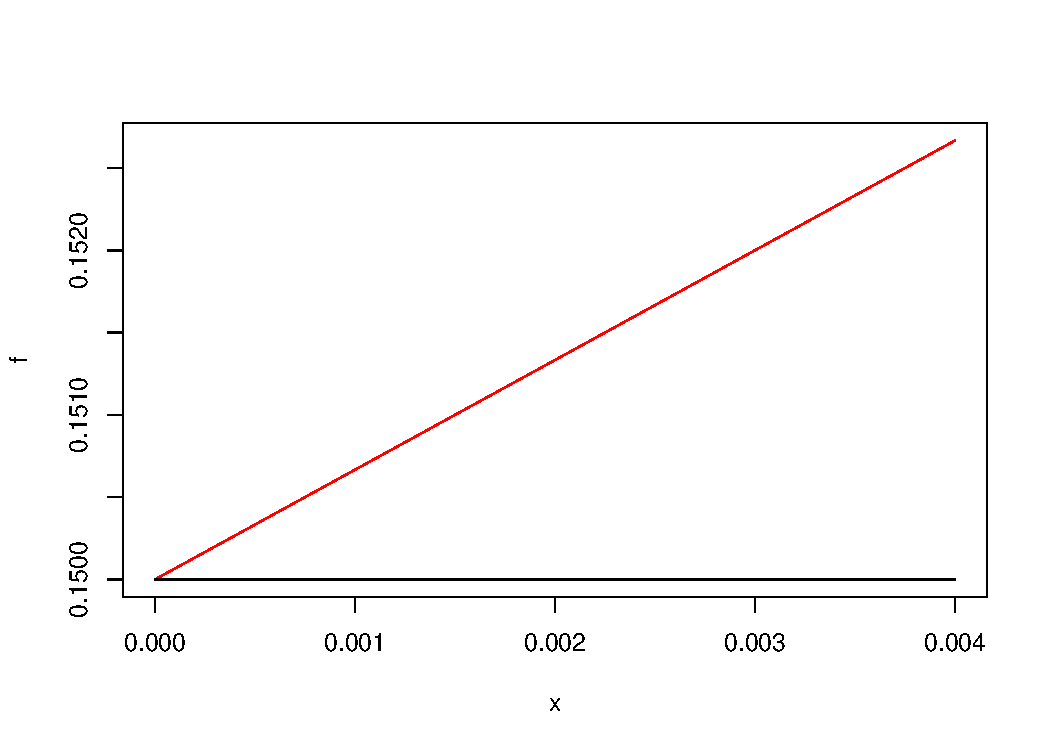
\includegraphics[scale=0.6]{para_approx.pdf}
With Paraxial Approximation focus point always becomes $0.15$ m, independent 
of where on the lins a beam parallel with the optic normal axis refract on the lens.
Mean while without the approximation it will drift futher away from the lins 
when the standard beam closes the edge of the lens.
 $$[placeholder]$$

\subsubsection{B: Material Replacement}
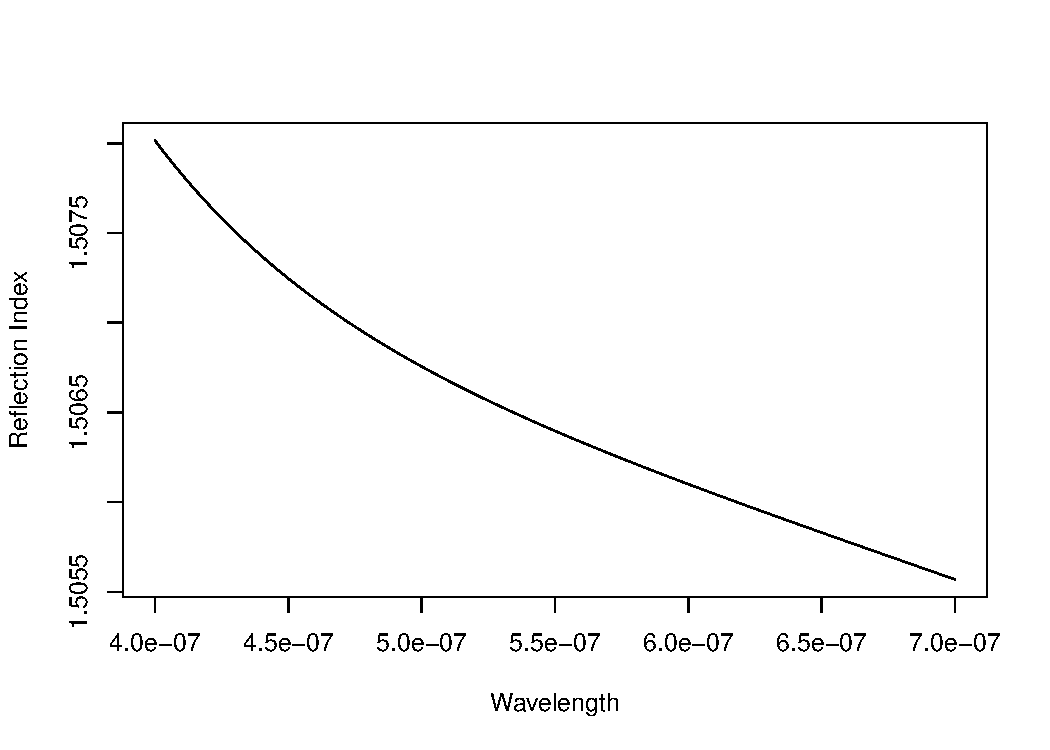
\includegraphics[scale=0.6]{BK7_index.pdf}
When plotting BK7 refraction index compared to wavelength of the incoming light,
the graph shows that $\Delta$ $0.0025$ in index between lowest value 
$400 nm$ and highest $700 nm$.
The function is close to liner at the high spectrum, which is wort noting.

\subsubsection{C: Chromatic Aborations}
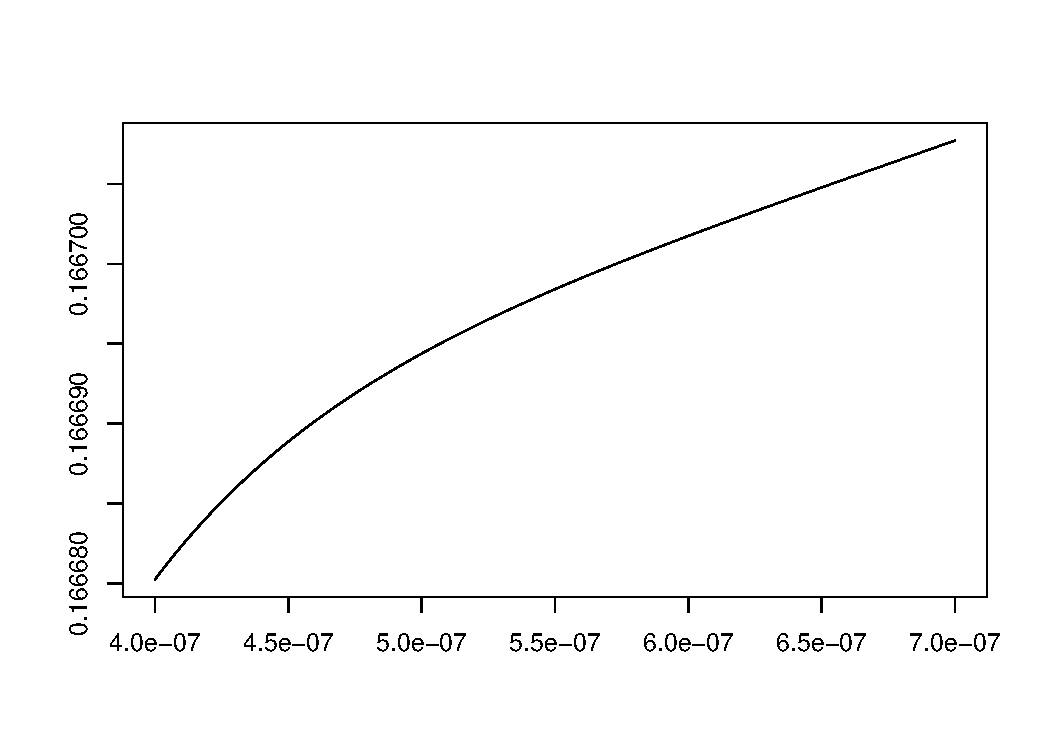
\includegraphics[scale=0.6]{BK7_abo.pdf}
Applying the BK7 material on the none Paraxial Approximated function, gives us
an $\Delta$ in focus point of close to $0.00028$. Generally close to $0.15$

\subsection{Conclusion and Commentary}
Replacement material $BK7$ has the properties to almost bring focus back to $0.15$, where it was when we applied Paraxial Approimation. 
Conclusion with the new material we can easy apply Paraxial Approximation
without to large errors in calculations, depending on specification limitation of cource. 

\section{Assignment 2: Laser Pulse}

\subsection{Implemation}

\subsection{Resultat}
\subsubsection{A: Nummeric Solution}

\subsubsection{B: Differential Plot}
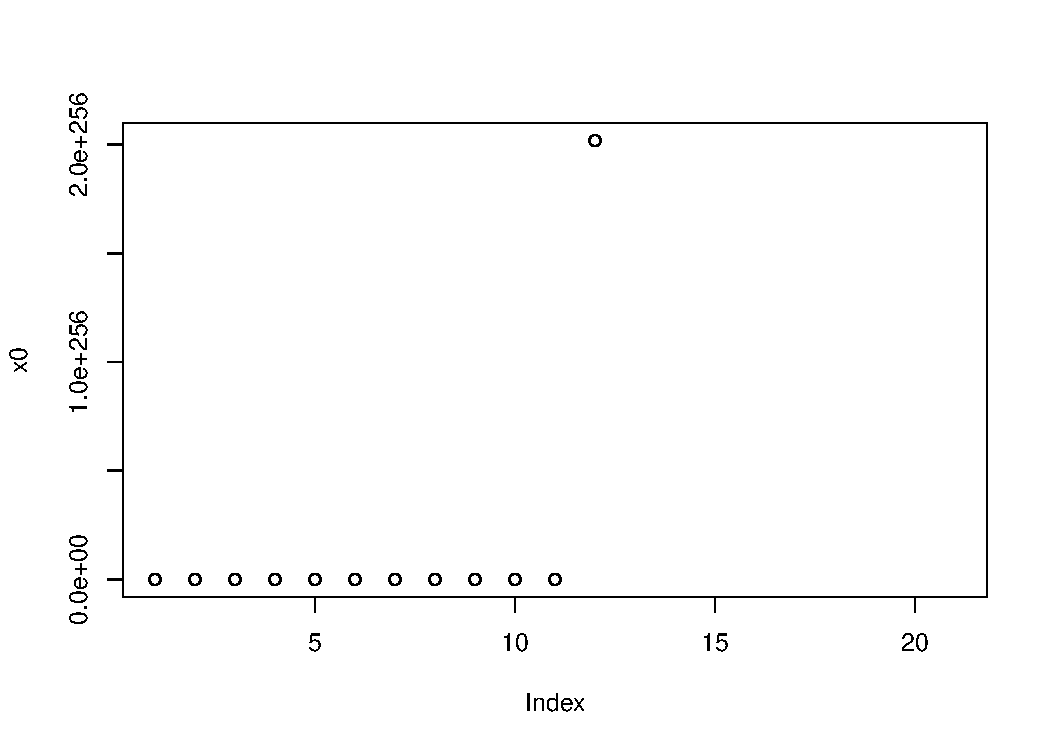
\includegraphics[scale=0.6]{N.pdf}

\subsection{Conclusion and Commentary}

\newpage
\appendix
\section{Implementation R Code}
\subsection{Assignment I:}
\label{1:gua}
\lstinputlisting[title=Guassian Function, numbers=left, keepspaces=true, firstline=7, lastline=15, language=R, basicstyle=\ttfamily\tiny]{datoruppgift.r}
\label{1:para}
\lstinputlisting[title=Paraxial Approximation, numbers=left, keepspaces=true, firstline=18, lastline=21, language=R, basicstyle=\ttfamily\tiny]{datoruppgift.r}
\label{1:nopara}
\lstinputlisting[title=No Paraxial Approximation, numbers=left, keepspaces=true, firstline=23, lastline=26, language=R, basicstyle=\ttfamily\tiny]{datoruppgift.r}
\label{1:BK7}
\lstinputlisting[title=BK7 refraction index, numbers=left, keepspaces=true, firstline=29, lastline=40, language=R, basicstyle=\ttfamily\tiny]{datoruppgift.r}
\subsection{Assignment II: }
\lstinputlisting[numbers=left, keepspaces=true, firstline=68, basicstyle=\ttfamily\tiny]{datoruppgift.r}
\end{document}
